\documentclass{source/Paper}
% !TEX program = xelatex
\major{}
\name{}
\articletitle{2024-2025学年电子电路基础期末考试}
\stuid{}
\college{信息与电子工程学院}
\date{\today}
\course{电子电路基础}
\instructor{}
\usepackage{amsmath}
\usepackage{tcolorbox}
\usepackage{xcolor}
\tcbuselibrary{breakable}
\begin{document}
\makeheader
\section{选择题(每题2分，共20分)}

    \subsection{下列哪一项是正确的？}
    A 不同频率激励源不能用叠加定理 

    B 电流先于电压是感性阻抗

    C 忘了… 

    D 电感电压先于电流，电容电压落后于电流
    \subsection{已知$\Delta$电阻网络的电阻每个均为60$\Omega$, 问Y形网络的每个电阻是多少？}
    \subsection{哪个点摆幅最大？}
    \begin{figure}[H]
        \centering
        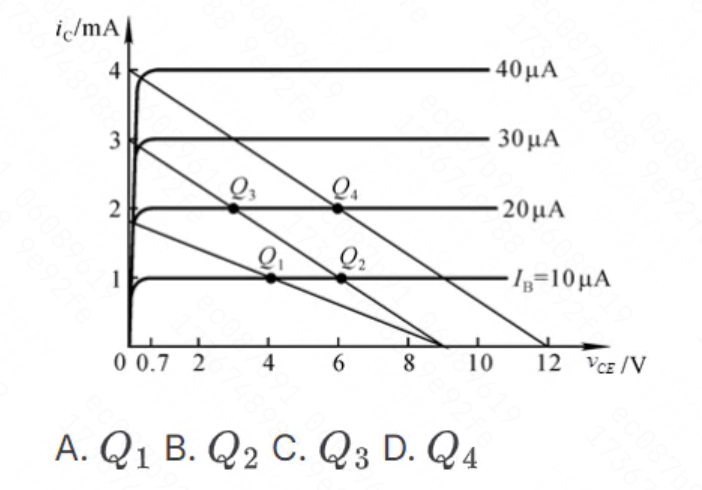
\includegraphics[width=0.5\textwidth]{image1.png}        
    \end{figure}
    \subsection{测量某放大电路负载开路时输出电压为 3 V，接入2$k\Omega$ 负载后，测得输出电压为 1 V，则该放大电路的输出电阻为?}
    A. 0.5 kΩ
    B. 1.0 kΩ
    C. 2.0 kΩ
    D. 4.0 kΩ
    \subsection{好像考了甲乙类/乙类的相位（很基础的那种）}
    \subsection{放大器深度负反馈的条件是?}
    A. $│1+AF│ \gg 1$ 
    B．$│A│ \gg 1$ 
    C．$│F│ \gg 1$ 
    D．$│1/F│ \gg 1$
    \subsection{求下面电路D1、D2的导通情况?}
    \begin{figure}[H]
        \centering
        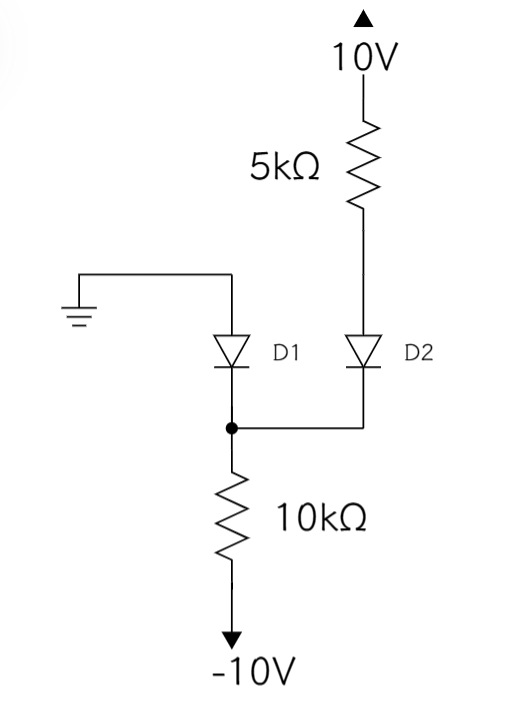
\includegraphics[width=0.5\textwidth]{image2.png}        
    \end{figure}
\section{填空题}
\subsection{理想运放虚短是因为（               ），虚断是因为（                 ）}
\subsection{}


\end{document}

